\documentclass[12pt,a4paper]{article}

\usepackage[utf8]{inputenc}
\usepackage[T1]{fontenc}
\usepackage{mathpazo}
\usepackage[margin=1.15in]{geometry}
\usepackage{setspace}
\usepackage{hyperref}
\usepackage{titlesec}
\usepackage{amsmath,amsthm,amssymb}
\usepackage{booktabs}
\usepackage{enumitem}
\usepackage{fancyhdr}
\usepackage{xcolor}
\usepackage{tcolorbox}
\usepackage{tikz}
\usepackage{array}
\usepackage{float}

\newtcolorbox{vizpanel}[1][]{
  colback=gray!4, colframe=gray!50!black,
  fonttitle=\bfseries, title={Visualization: #1},
  sharp corners, boxrule=0.5pt
}

\hypersetup{colorlinks=true, linkcolor=blue!70!black, citecolor=black, urlcolor=blue!70!black}

\titleformat{\section}{\large\bfseries}{\thesection}{0.7em}{}
\titleformat{\subsection}{\normalsize\bfseries}{\thesubsection}{0.7em}{}
\titleformat{\subsubsection}{\normalsize\itshape}{\thesubsubsection}{0.7em}{}

\newtheorem{definition}{Definition}[section]
\newtheorem{proposition}[definition]{Proposition}
\newtheorem{theorem}[definition]{Theorem}
\newtheorem{lemma}[definition]{Lemma}
\newtheorem{corollary}[definition]{Corollary}
\newtheorem{example}[definition]{Example}
\theoremstyle{remark}
\newtheorem{remark}[definition]{Remark}

\newcommand{\R}{\mathbb{R}}
\newcommand{\ones}{\mathbf{1}}
\newcommand{\x}{\mathbf{x}}
\newcommand{\y}{\mathbf{y}}
\newcommand{\K}{\mathbf{K}}
\newcommand{\bsigma}{\boldsymbol{\sigma}}
\newcommand{\btheta}{\boldsymbol{\theta}}
\DeclareMathOperator*{\argmax}{arg\,max}

\newtcolorbox{intuition}[1][]{
  colback=blue!3, colframe=blue!40!black,
  fonttitle=\bfseries, title={Intuition: #1},
  sharp corners, boxrule=0.5pt
}

\newtcolorbox{keyinsight}[1][]{
  colback=orange!5, colframe=orange!60!black,
  fonttitle=\bfseries, title={Key Structural Insight},
  sharp corners, boxrule=0.5pt
}

\newtcolorbox{prebisch}[1][]{
  colback=green!3, colframe=green!40!black,
  fonttitle=\bfseries, title={Prebisch Connection: #1},
  sharp corners, boxrule=0.5pt
}

\setlength{\parindent}{1.5em}
\onehalfspacing

\setlength{\headheight}{14pt}
\pagestyle{fancy}
\fancyhf{}
\fancyhead[L]{\small\itshape Chapter 3: Growth and Distribution in Matrix Form}
\fancyhead[R]{\small\thepage}
\renewcommand{\headrulewidth}{0.4pt}

\title{\vspace{-1cm}\textbf{Chapter 3} \\[0.5em]
\LARGE Growth and Distribution in Matrix Form \\[0.3em]
\large\textit{Why Growth Makes Some Countries Rich and Others More Unequal}}
\author{}
\date{}

\begin{document}

\maketitle
\thispagestyle{fancy}

\begin{quote}
\textit{``Los enormes beneficios que derivan de la creciente productividad no han llegado a la periferia en medida comparable a la que han logrado disfrutar las poblaciones de los grandes pa\'{i}ses industriales. De ah\'{i} las diferencias tan acentuadas en los niveles de vida de las masas de \'{e}stos y de aqu\'{e}llos y las notorias discrepancias entre sus respectivas fuerzas de capitalizaci\'{o}n.''}\\[0.3em]
\textnormal{[``The enormous benefits derived from increasing productivity have not reached the periphery in a measure comparable to that enjoyed by the peoples of the great industrial countries. Hence the great differences in standards of living, and the manifest discrepancies in their respective capacities for capital accumulation.'']}\\
\hfill --- Ra\'{u}l Prebisch, \textit{El desarrollo econ\'{o}mico de la Am\'{e}rica Latina} (1949)
\end{quote}

\vspace{0.5em}

\begin{quote}
\textit{``Che boludo, it's obvious.''}\\[0.3em]
\hfill --- What Prebisch would have said about this chapter
\end{quote}

\vspace{1em}

Prebisch saw it without the math: growth in the periphery does not work the same way as growth in the center, and the difference is structural. The production structure of the center---diversified, interconnected, industrialized---propagates productivity gains internally, raising wages and living standards broadly. The production structure of the periphery---concentrated in primary commodities, weakly linked internally, dependent on imported technology---leaks productivity gains outward through deteriorating terms of trade, leaving internal inequality unchanged or worse.

This chapter gives Prebisch his eigenvalues.

We develop growth theory in matrix form, starting from the standard Solow model (one sector, one country, growth converges to a steady state) and progressively introducing the structural elements that make growth in the periphery different from growth in the center. The key mathematical object is the production network $A$---the input-output matrix from Chapter~1---now embedded in a dynamic growth model where the structure of $A$ determines not just who produces what today but how productivity gains propagate across sectors over time.

The central result: whether growth reduces or increases inequality depends on the \textit{spectral properties} of $A$. When $A$ is well-connected (strong inter-sectoral linkages, large spectral gap), growth propagates and converges. When $A$ is block-diagonal (disconnected sectors, small spectral gap), growth concentrates in the modern sector and does not reach the traditional sector. Pinto's structural heterogeneity is a spectral property.


%% =====================================================================
\section{The Standard Story: One Sector, One Country}
\label{sec:solow}
%% =====================================================================

\subsection{Solow in One Paragraph}

The Solow growth model says: a country accumulates capital, capital produces output, output is split between consumption and saving, and saving becomes next period's capital. The economy converges to a steady state where capital per worker is constant and output grows only through technological progress.

The model has one sector, one representative agent, and one production function: $Y_t = K_t^\alpha (A_t L_t)^{1-\alpha}$, where $K$ is capital, $L$ is labor, $A$ is technology, and $\alpha \in (0,1)$ is the capital share. The savings rate $s$ is exogenous. Capital accumulates as $K_{t+1} = sY_t + (1-\delta)K_t$.

In per-effective-worker terms ($k = K/(AL)$), the dynamics reduce to one equation:
\begin{equation}\label{eq:solow}
k_{t+1} = \frac{s k_t^\alpha + (1-\delta)k_t}{(1+g)(1+n)},
\end{equation}
where $g$ is the growth rate of technology and $n$ is population growth. The steady state $k^*$ satisfies $sf(k^*) = (\delta + g + n)k^*$.

\begin{intuition}[What Solow gets right and what it misses]
Solow gets convergence right: poor countries with low $k$ have high marginal product of capital, invest at the same rate $s$, and grow faster until they catch up. This predicts convergence---and conditional convergence (controlling for $s$, $\delta$, $n$) is one of the most robust findings in empirical growth.

What Solow misses is everything structural. There is one sector, so there is no structural heterogeneity. There is one savings rate, so there is no differential accumulation by group. There is one production function, so there are no inter-sectoral linkages, no Leontief multipliers, no question of whether growth in mining propagates to agriculture. The country is a point, not a structure. Prebisch would say: this describes Sweden, not Bolivia.
\end{intuition}


\subsection{Solow with Two Groups: The OLG Version}

To introduce structure, we move from the Solow model to the overlapping-generations (OLG) framework, where savings decisions are made by \textit{different groups} with \textit{different parameters}.

\begin{example}[A Two-Group Economy]\label{ex:two_group}
Consider an economy with two groups: $M$ (men) and $F$ (women), each comprising half the population. Each agent lives two periods: young (work, earn, save) and old (consume savings).

A young agent of group $g \in \{M, F\}$ has utility over young and old consumption:
\begin{equation}\label{eq:OLG_utility}
U^g = \ln(c^{g,y}) + \theta^g \ln(c^{g,o}),
\end{equation}
where $\theta^g > 0$ is the \textbf{patience parameter}---how much group $g$ values future consumption relative to present consumption.

The budget constraints are $c^{g,y} + s^g = w_t$ (young: consume or save out of wage income) and $c^{g,o} = (1 + r_{t+1})s^g$ (old: consume return on savings). The optimal savings rate is:
\begin{equation}\label{eq:savings_rate}
\sigma(\theta^g) = \frac{\theta^g}{1 + \theta^g}.
\end{equation}

A group with higher $\theta$ (more patient) saves a larger fraction of income. If $\theta^M = \theta^F$ (same patience), both groups save the same share and the economy behaves like standard Solow. If $\theta^M > \theta^F$---if men are more patient than women, or more precisely, if the structure has produced men who value future consumption more---then men save more, accumulate more, and the wealth gap widens over time.
\end{example}

Aggregate capital next period is:
\begin{equation}\label{eq:K_OLG}
K_{t+1} = \frac{1}{2}\bigl[\sigma(\theta^M_t) + \sigma(\theta^F_t)\bigr](1-\alpha)K_t^\alpha.
\end{equation}

This is the Solow model with a twist: the aggregate savings rate depends on the \textit{composition} of the population. If the two groups have different patience parameters, the savings rate---and therefore the growth path---depends on who has what $\theta$.

\begin{intuition}[Where does $\theta$ come from?]
In the standard OLG model, $\theta^g$ is given. Men and women are either equally patient or not, and the model does not ask why. In the formation model (Chapter~10), $\theta^g$ is produced by the park: the developmental environment determines how much each group values future consumption, investment, and career building. Women raised in a normative environment where female economic participation is invisible or discouraged will have lower $\theta^F$---not because of biology but because the signal structure of the park made future consumption appear less attainable or less valuable.

For now, $\theta^g$ is a parameter. Later, it becomes an output of $W^I$.
\end{intuition}


%% =====================================================================
\section{Multi-Sector Growth: The Production Network}
\label{sec:multi_sector}
%% =====================================================================

Now we introduce multiple sectors. This is where the Leontief system from Chapter~1 becomes dynamic.

\subsection{A Story: Gas and Quinoa}

Bolivia has two economies. The first is the gas economy: capital-intensive, high-productivity, connected to global commodity markets, responsible for roughly 30\% of GDP and 50\% of export revenues, employing approximately 1\% of the labor force. The second is the quinoa economy (and potatoes, and llamas, and informal commerce): labor-intensive, low-productivity, disconnected from global markets, employing the vast majority of the population.

A dollar of investment in the gas sector produces output that is sold internationally, generates fiscal revenue, and feeds back into the gas sector (maintenance, exploration, expansion). Very little of it flows to quinoa farmers. A dollar of investment in quinoa production feeds local consumption, local transport, local markets---but generates negligible fiscal revenue and zero export earnings.

This is structural heterogeneity. And the question is: if the gas sector grows at 5\% per year for a decade, does the quinoa economy grow?

The answer depends on the structure of $A$---the input-output matrix. If the gas sector buys inputs from the domestic economy (backward linkages) and sells intermediate products to domestic manufacturers (forward linkages), then gas growth propagates. If the gas sector imports its inputs and exports its output, with no domestic linkages, then gas growth is an enclave: it enriches the gas sector and the treasury without touching the quinoa economy.

\begin{prebisch}[The enclave economy]
This is exactly Prebisch's center-periphery argument applied within a country. The gas sector is the ``center'' of the Bolivian economy---high productivity, strong international linkages, favorable terms of trade (when commodity prices are high). The traditional sector is the ``periphery''---low productivity, weak linkages, dependent on domestic demand. Pinto's contribution was to see that this center-periphery structure exists \textit{inside} peripheral countries, not just between countries. Bolivia is peripheral in the global economy \textit{and} internally heterogeneous. The gas sector's relationship to the quinoa sector replicates, at national scale, the center's relationship to the periphery at global scale.
\end{prebisch}


\subsection{The Multi-Sector Solow Model}

Consider $N$ sectors, each with its own capital stock $K_{it}$, labor force $L_i$, and production function. Sector $i$ produces:
\begin{equation}\label{eq:sector_production}
Y_{it} = K_{it}^{\alpha_i} L_i^{1-\alpha_i} + \gamma \sum_{j=1}^N W^P_{ij} Y_{jt},
\end{equation}
where the second term captures production spillovers: sector $i$'s output benefits from sector $j$'s output, weighted by $W^P_{ij}$ (the input-output coefficient).

In matrix form, stacking all sectors:
\begin{equation}\label{eq:output_system}
\mathbf{Y}_t = \mathbf{f}(\K_t, \mathbf{L}) + \gamma W^P \mathbf{Y}_t,
\end{equation}
where $\mathbf{f}$ is the vector of Cobb-Douglas production functions. Solving for $\mathbf{Y}_t$ (as in Chapter~1):
\begin{equation}\label{eq:output_solution}
\mathbf{Y}_t = (I - \gamma W^P)^{-1}\mathbf{f}(\K_t, \mathbf{L}).
\end{equation}

This is the Leontief system made dynamic: at each period $t$, output is determined by capital (which accumulates) filtered through the production network (which amplifies through the Leontief inverse).

Capital accumulates sector by sector:
\begin{equation}\label{eq:capital_dynamics}
K_{i,t+1} = s_i Y_{it} + (1-\delta_i) K_{it},
\end{equation}
where $s_i$ is sector $i$'s savings (reinvestment) rate and $\delta_i$ is depreciation. In matrix form:
\begin{equation}\label{eq:capital_vector}
\K_{t+1} = S \mathbf{Y}_t + (I - \Delta)\K_t,
\end{equation}
where $S = \text{diag}(s_1, \ldots, s_N)$ and $\Delta = \text{diag}(\delta_1, \ldots, \delta_N)$.

Substituting the output equation:
\begin{equation}\label{eq:growth_system}
\K_{t+1} = S(I - \gamma W^P)^{-1}\mathbf{f}(\K_t, \mathbf{L}) + (I - \Delta)\K_t.
\end{equation}

\begin{keyinsight}
Equation~\eqref{eq:growth_system} is the multi-sector growth equation. It says: next period's capital depends on this period's capital, transformed by two structural objects:
\begin{itemize}
\item $(I - \gamma W^P)^{-1}$: the Leontief inverse, which amplifies each sector's output through inter-sectoral linkages.
\item $S$: the savings matrix, which determines how much of each sector's output is reinvested.
\end{itemize}

The \textit{structure} of growth---which sectors grow, how fast, and whether growth spreads across sectors---is governed by the interaction of these two matrices.
\end{keyinsight}


\subsection{The Steady State}

At the steady state $\K^*$, capital is constant: $\K^* = S(I - \gamma W^P)^{-1}\mathbf{f}(\K^*, \mathbf{L}) + (I - \Delta)\K^*$. For Cobb-Douglas production ($f_i = K_i^\alpha L_i^{1-\alpha}$ with common $\alpha$), this simplifies to:
\begin{equation}
\Delta \K^* = S(I - \gamma W^P)^{-1}\mathbf{f}(\K^*, \mathbf{L}).
\end{equation}

Finding $\K^*$ is a fixed-point problem. For the linear case ($\alpha = 1$, which makes $f_i = K_i$), the system becomes:
\begin{equation}
\K^* = [I - (I - \Delta)^{-1}S(I - \gamma W^P)^{-1}]^{-1} \cdot \mathbf{0},
\end{equation}
which is degenerate (trivial steady state at zero without technological progress). The interesting dynamics are in the transition path, which is governed by the eigenvalues of the \textit{growth mapping} $G = (I - \Delta) + S(I - \gamma W^P)^{-1}F'(\K^*)$, where $F'$ is the Jacobian of the production function.


%% =====================================================================
\section{When Does Growth Reduce Inequality? The Kuznets Question}
\label{sec:kuznets}
%% =====================================================================

\subsection{The Standard Answer}

Simon Kuznets (1955) proposed that inequality first rises and then falls with development---the ``inverted-U'' hypothesis. The mechanism: early industrialization pulls workers from a low-inequality agricultural sector into a high-inequality industrial sector, raising between-sector inequality. Eventually, as most workers have moved, within-sector inequality dominates and falls.

The inverted-U has been one of the most tested hypotheses in economics. The evidence is mixed at best: cross-country data show no robust inverted-U, and the within-country trajectories vary enormously. Some countries (South Korea, Taiwan) grew rapidly and reduced inequality. Others (Brazil in the 1960s-70s, Bolivia, Nigeria) grew and saw inequality rise. Others (many sub-Saharan African countries) did not grow and saw inequality rise anyway.

The matrix framework explains why: it depends on $W^P$.

\subsection{The Structural Answer: It Depends on $W^P$}

\begin{example}[Two Economies, Same Technology, Different $W^P$]\label{ex:two_WP}
Consider two economies, each with $N = 2$ sectors: Modern ($M$) and Traditional ($T$). Both have the same technology:
\begin{equation}
Y_M = K_M^{0.4} L_M^{0.6}, \qquad Y_T = K_T^{0.3} L_T^{0.7}.
\end{equation}

Modern is more capital-intensive ($\alpha_M = 0.4 > \alpha_T = 0.3$). Both sectors have savings rate $s = 0.2$ and depreciation $\delta = 0.05$.

\textbf{Economy A (Connected):} Strong inter-sectoral linkages.
\begin{equation}
W^P_A = \begin{pmatrix} 0.10 & 0.25 \\ 0.20 & 0.10 \end{pmatrix}.
\end{equation}
Modern uses Traditional inputs ($W^P_{M,T} = 0.25$): factories buy agricultural raw materials. Traditional uses Modern inputs ($W^P_{T,M} = 0.20$): farmers buy manufactured fertilizer and equipment.

\textbf{Economy B (Disconnected):} Weak inter-sectoral linkages.
\begin{equation}
W^P_B = \begin{pmatrix} 0.10 & 0.02 \\ 0.02 & 0.10 \end{pmatrix}.
\end{equation}
The sectors barely interact. Modern imports its inputs and exports its output. Traditional produces for local consumption.

Now give both economies a productivity shock in the Modern sector: $A_M$ doubles.
\end{example}

\begin{example}[Continued: The Propagation]\label{ex:propagation}
The Leontief inverse for Economy A:
\begin{equation}
L_A = (I - \gamma W^P_A)^{-1} \approx \begin{pmatrix} 1.05 & 0.27 \\ 0.21 & 1.05 \end{pmatrix} \quad (\text{with } \gamma = 1).
\end{equation}

A productivity shock in Modern ($\Delta Y_M = 1$) generates total output increase of $1.05$ in Modern (direct + own-sector feedback) and $0.21$ in Traditional (cross-sector spillover). The Traditional sector benefits because it sells inputs to Modern.

The Leontief inverse for Economy B:
\begin{equation}
L_B = (I - \gamma W^P_B)^{-1} \approx \begin{pmatrix} 1.01 & 0.02 \\ 0.02 & 1.01 \end{pmatrix}.
\end{equation}

The same shock in Modern generates $1.01$ in Modern and only $0.02$ in Traditional. The spillover is negligible. Growth in Modern stays in Modern.

After 10 periods of compounding, Economy A shows both sectors growing (Traditional pulled up by its linkages to Modern). Economy B shows Modern growing and Traditional stagnant---the productivity gap \textit{widens} with growth.
\end{example}

\begin{proposition}[Growth Propagation and the Spectral Gap]\label{prop:propagation}
Consider the multi-sector growth model~\eqref{eq:growth_system} with $N$ sectors and production network $W^P$. A productivity shock in sector $j$ propagates to sector $i$ with magnitude proportional to the $(i,j)$-th entry of the Leontief inverse $(I - \gamma W^P)^{-1}$.

The average cross-sector propagation is bounded by:
\begin{equation}
\frac{1}{N(N-1)} \sum_{i \neq j} \ell_{ij} \leq \frac{\gamma \|W^P\|}{1 - \gamma\rho(W^P)},
\end{equation}
where $\ell_{ij}$ are off-diagonal entries of the Leontief inverse and $\rho(W^P)$ is the spectral radius. The propagation is small when $\gamma\rho(W^P)$ is small (weak linkages) and large when $\gamma\rho(W^P)$ is close to 1 (strong linkages, near the productivity boundary).
\end{proposition}

\begin{intuition}[What this says in words]
Whether growth in one sector helps another sector depends on how connected they are in the production network. If the Leontief inverse has large off-diagonal entries (sectors are strongly linked), growth propagates. If the off-diagonal entries are small (sectors are weakly linked), growth concentrates. The spectral radius of $W^P$ governs the overall strength of inter-sectoral transmission.
\end{intuition}

\begin{proof}
The Leontief inverse is $(I - \gamma W^P)^{-1} = \sum_{k=0}^\infty \gamma^k (W^P)^k$. The off-diagonal entries are $\ell_{ij} = \sum_{k=1}^\infty \gamma^k (W^P)^k_{ij}$ (the $k=0$ term is $I$, contributing only to the diagonal). Each power $(W^P)^k_{ij}$ represents paths of length $k$ from $j$ to $i$, and satisfies $|(W^P)^k_{ij}| \leq \rho(W^P)^k$ for the spectral radius. Summing the geometric bound:
\begin{equation}
\ell_{ij} \leq \sum_{k=1}^\infty \gamma^k \rho(W^P)^k = \frac{\gamma\rho(W^P)}{1 - \gamma\rho(W^P)}.
\end{equation}
Averaging over the $N(N-1)$ off-diagonal entries gives the bound. For the norm bound, use $|(W^P)^k_{ij}| \leq \|W^P\|^k$ and $\|(W^P)^k\| \leq \|W^P\|^k$.
\end{proof}


%% =====================================================================
\section{Structural Heterogeneity: The Block-Diagonal Economy}
\label{sec:heterogeneity}
%% =====================================================================

\subsection{Pinto's Diagnosis}

An\'{i}bal Pinto observed in the 1960s that Latin American economies were not uniformly ``underdeveloped.'' They contained a modern sector with productivity levels comparable to the center, coexisting with a traditional sector with productivity levels comparable to the 19th century. The gap between sectors---within the same country---was often larger than the gap between the modern sector and the developed world.

This was not a transitional phase. It was a stable configuration. Growth did not close the gap; it widened it. The modern sector absorbed capital and technology, grew rapidly, and became more productive. The traditional sector absorbed labor, grew slowly or not at all, and stagnated. The structural disconnection between them prevented the propagation that would have equalized productivity.

We now formalize this.

\begin{definition}[Structural Heterogeneity]\label{def:heterogeneity}
An economy with production network $W^P$ has \textbf{structural heterogeneity of degree $k$} if $W^P$ is approximately block-diagonal with $k$ blocks:
\begin{equation}\label{eq:block_diagonal}
W^P \approx \begin{pmatrix} W^P_{11} & \varepsilon_{12} \\ \varepsilon_{21} & W^P_{22} \end{pmatrix},
\end{equation}
where $W^P_{11}$ and $W^P_{22}$ are the within-block (within-sector) linkage matrices and $\varepsilon_{12}, \varepsilon_{21}$ are the cross-block linkages, with $\|\varepsilon_{12}\|, \|\varepsilon_{21}\| \ll \|W^P_{11}\|, \|W^P_{22}\|$.

Degree $k = 1$: the economy is structurally integrated (one block). Degree $k = 2$: the economy has a dual structure (Pinto's case). Degree $k > 2$: multiple disconnected sectors.
\end{definition}

\begin{example}[Bolivia: A Degree-2 Economy]\label{ex:bolivia}
Bolivia's production structure can be stylized as two blocks:

\textbf{Block 1 (Modern):} Gas extraction, mining, large-scale agriculture (soybeans), financial services. High capital intensity, high productivity, strong linkages to global markets, weak linkages to the domestic traditional sector.

\textbf{Block 2 (Traditional):} Subsistence agriculture (quinoa, potatoes, llamas), informal commerce, small-scale manufacturing, domestic services. Labor-intensive, low productivity, strong internal linkages (farmers sell to local markets, local markets sell to local consumers), negligible linkages to the modern sector.

The stylized $W^P$:
\begin{equation}
W^P_{\text{Bolivia}} \approx \begin{pmatrix} 0.15 & 0.03 \\ 0.02 & 0.20 \end{pmatrix}.
\end{equation}

Within the modern sector, linkages are moderate ($0.15$): gas companies buy services from financial firms, mining needs transport. Within the traditional sector, linkages are strong ($0.20$): the farmer sells to the market seller who buys from the small manufacturer. But cross-sector linkages are tiny ($0.03$ and $0.02$): the gas sector imports its equipment from Brazil, not from Bolivian workshops; the quinoa farmer does not sell to the gas company cafeteria.

The Leontief inverse:
\begin{equation}
L \approx \begin{pmatrix} 1.18 & 0.04 \\ 0.03 & 1.25 \end{pmatrix}.
\end{equation}

A productivity shock in the gas sector (column 1) generates 1.18 units of output in the modern sector and 0.03 in the traditional sector. Almost none of the growth propagates. The enclave multiplier is 1.21; of this, 97.5\% stays in the modern sector.

Compare with a hypothetical connected Bolivia where cross-sector linkages are $0.15$ instead of $0.03$:
\begin{equation}
W^P_{\text{connected}} = \begin{pmatrix} 0.15 & 0.15 \\ 0.15 & 0.20 \end{pmatrix}, \quad L_{\text{connected}} \approx \begin{pmatrix} 1.26 & 0.23 \\ 0.21 & 1.33 \end{pmatrix}.
\end{equation}

Now the same gas shock generates 0.21 units in the traditional sector---seven times more propagation. The multiplier rises to 1.47, with 14\% reaching the traditional sector.
\end{example}

\begin{prebisch}[The multiplier gap is the development gap]
The difference between the two Bolivias above is not technology, not savings rates, not human capital, not institutions in the Acemoglu-Robinson sense. It is the \textit{structure of inter-sectoral linkages}---the topology of $W^P$. Both economies have the same production functions, the same capital, the same labor. They differ only in how connected the sectors are. And this difference produces, over time, radically different development trajectories.

This is Prebisch's core argument, formalized: the terms of trade deterioration is a consequence of the periphery's weak structural linkages. When the center grows, its interconnected production structure amplifies the growth internally. When the periphery grows, its disconnected structure leaks the growth externally (through commodity export revenues that purchase imported manufactures) without amplifying it internally.

The multiplier gap---the difference in off-diagonal entries of the Leontief inverse between a connected and a disconnected economy---\textit{is} the development gap. It is computable. It is a property of $W^P$. And it can be changed.
\end{prebisch}

\begin{vizpanel}{Bolivia's two possible Leontief inverses}
\begin{center}
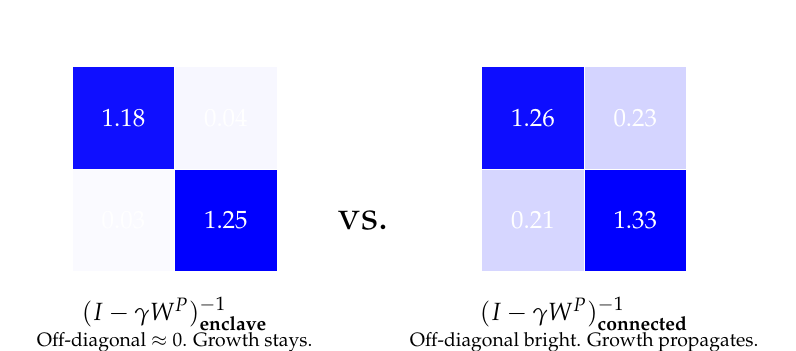
\begin{tikzpicture}[scale=1]
\def\s{1.3}
%% Disconnected Bolivia: L = (1.18, 0.04; 0.03, 1.25)
\foreach \i/\j/\v/\lab in {1/1/94/1.18, 1/2/3/0.04, 2/1/2/0.03, 2/2/100/1.25} {
  \fill[blue!\v, draw=white, line width=0.3pt]
    ({(\j-1)*\s}, {(2-\i)*\s}) rectangle +(\s,\s);
  \node[font=\small, white] at ({(\j-0.5)*\s}, {(2-\i+0.5)*\s}) {\lab};
}
\node[below, font=\small\bfseries] at ({\s}, -0.2) {$(I-\gamma W^P)^{-1}_{\text{enclave}}$};
\node[below, font=\scriptsize] at ({\s}, -0.65) {Off-diagonal $\approx 0$. Growth stays.};

\node[font=\Large] at (3.7, 0.65) {vs.};

%% Connected Bolivia: L = (1.26, 0.23; 0.21, 1.33)
\begin{scope}[xshift=5.2cm]
\foreach \i/\j/\v/\lab in {1/1/95/1.26, 1/2/17/0.23, 2/1/16/0.21, 2/2/100/1.33} {
  \fill[blue!\v, draw=white, line width=0.3pt]
    ({(\j-1)*\s}, {(2-\i)*\s}) rectangle +(\s,\s);
  \node[font=\small, white] at ({(\j-0.5)*\s}, {(2-\i+0.5)*\s}) {\lab};
}
\node[below, font=\small\bfseries] at ({\s}, -0.2) {$(I-\gamma W^P)^{-1}_{\text{connected}}$};
\node[below, font=\scriptsize] at ({\s}, -0.65) {Off-diagonal bright. Growth propagates.};
\end{scope}
\end{tikzpicture}
\end{center}
\vspace{-0.5em}
\small Same economy, same production functions, same capital, same labor. The only difference is the off-diagonal entries of $W^P$ (0.03 vs.\ 0.15). Left: the Leontief inverse is nearly diagonal --- a gas shock generates 0.03 in the traditional sector. Right: the same shock generates 0.21 --- seven times more. The dark off-diagonal squares on the left are the trickle-down problem in two pixels.
\end{vizpanel}


\subsection{The Spectral Signature of Heterogeneity}

\begin{proposition}[Spectral Properties of Block-Diagonal Economies]\label{prop:block_spectral}
Let $W^P$ be approximately block-diagonal with $k = 2$ blocks as in~\eqref{eq:block_diagonal}. Then:
\begin{enumerate}
\item The eigenvalues of $W^P$ are approximately the union of the eigenvalues of $W^P_{11}$ and $W^P_{22}$, plus perturbation terms of order $\|\varepsilon\|$.
\item The spectral gap $\Gamma(W^P) = \rho(W^P) - |\lambda_2(W^P)|$ is small when the two blocks have similar spectral radii: $\Gamma \approx |\rho(W^P_{11}) - \rho(W^P_{22})| + O(\|\varepsilon\|)$.
\item The Perron eigenvector of $W^P$ is approximately block-localized: it assigns most weight to the block with the larger spectral radius (the more productive/connected sector) and little weight to the other.
\end{enumerate}
\end{proposition}

\begin{intuition}[What this says in words]
A block-diagonal economy has a small spectral gap. And from Chapter~1 (Proposition~1B.1 in the appendix), a small spectral gap means: slow convergence, persistent asymmetries, and the possibility of extreme power concentration. In terms of growth: a block-diagonal production structure means that shocks propagate slowly between blocks, productivity differences persist across sectors, and the benefits of growth accrue primarily to the block with the higher spectral radius (the modern sector).

A connected economy has a large spectral gap. Growth propagates fast, sectoral differences converge, and the benefits are distributed broadly.

The spectral gap of $W^P$ is a single number that summarizes Pinto's entire structural heterogeneity argument.
\end{intuition}

\begin{proof}[Proof sketch]
(1) is a standard result in matrix perturbation theory (see Appendix~3A). If $W^P = \text{diag}(W^P_{11}, W^P_{22}) + E$ where $E$ is the off-diagonal block, then by the Bauer-Fike theorem, the eigenvalues of $W^P$ lie within $\|E\|$ of the eigenvalues of the block-diagonal part.

(2) follows because the two largest eigenvalues of the block-diagonal part are $\rho(W^P_{11})$ and $\rho(W^P_{22})$. If these are close, $\Gamma$ is small. The perturbation $E$ shifts both by order $\|E\|$.

(3) The Perron eigenvector of a block-diagonal matrix assigns weight only within the block that achieves $\rho$. The perturbation $E$ ``leaks'' some weight to the other block, but the leakage is proportional to $\|E\|/\Gamma$---small when $\|E\|$ is small.
\end{proof}


%% =====================================================================
\section{Does Growth Trickle Down? A Formal Answer}
\label{sec:trickle}
%% =====================================================================

\subsection{The Trickle-Down Hypothesis in Matrix Form}

The ``trickle-down'' hypothesis says: growth in the modern sector benefits the traditional sector through market linkages---increased demand for traditional products, higher wages that spread through labor mobility, technology transfer. In our framework, trickle-down is the claim that the off-diagonal entries of the Leontief inverse are large enough that modern-sector growth significantly raises traditional-sector output.

\begin{proposition}[The Trickle-Down Condition]\label{prop:trickle}
Growth in sector $j$ (the modern sector) ``trickles down'' to sector $i$ (the traditional sector) if and only if:
\begin{equation}\label{eq:trickle}
\ell_{ij} = [(I - \gamma W^P)^{-1}]_{ij} > \tau,
\end{equation}
where $\tau > 0$ is a threshold representing ``economically meaningful'' propagation. This is equivalent to requiring that there exists a chain of production linkages from $j$ to $i$ with sufficient cumulative strength.
\end{proposition}

\begin{intuition}[When does trickle-down fail?]
Trickle-down fails when $\ell_{ij}$ is small---when the Leontief inverse has small off-diagonal entries. This happens in three cases:
\begin{enumerate}
\item \textbf{Weak direct linkages}: $W^P_{ij}$ is small (the traditional sector does not sell inputs to the modern sector and does not buy its outputs).
\item \textbf{Weak indirect linkages}: there is no chain of intermediate sectors connecting $j$ to $i$ with sufficient strength. All paths through the network from $j$ to $i$ pass through weak links.
\item \textbf{The enclave}: the modern sector is connected to the \textit{global} economy but disconnected from the \textit{domestic} economy. Its linkages point outward (imports, exports) rather than inward (domestic input purchases, domestic sales).
\end{enumerate}

Bolivia's gas sector fails on all three counts. It does not buy inputs from the domestic traditional sector (case 1). There are no intermediate sectors linking gas to quinoa (case 2). Its linkages are to Brazilian pipeline operators and international commodity markets, not to Bolivian workshops (case 3).
\end{intuition}

\subsection{The Transfer Perversity Result}

Here is where the formation model connects to the growth model. Suppose the government, observing that gas growth does not trickle down, intervenes with a fiscal transfer: tax the modern sector and redistribute to the traditional sector. (This is, in essence, what Bolivia has done since 2006 with gas revenue-funded transfers like Renta Dignidad and Bono Juancito Pinto.)

\begin{proposition}[Transfer Perversity Under Structural Heterogeneity]\label{prop:transfer_perversity}
In a block-diagonal economy with structural heterogeneity, an unconditional transfer $\tau$ from the modern sector to the traditional sector:
\begin{enumerate}
\item \textbf{Raises traditional-sector income} (direct effect: $+\tau$).
\item \textbf{Raises traditional-sector capital} (through higher savings: $\Delta K_T = s_T \tau$).
\item \textbf{Lowers the modern-sector wage premium} (by raising traditional-sector productivity relative to the gap that motivates sector-switching).
\item \textbf{Weakens the signal for modern-sector investment} (the return differential between sectors narrows).
\item \textbf{Makes the traditional sector more attractive relative to the modern sector}, reducing the incentive for structural transformation.
\end{enumerate}

The net effect can be perverse: the transfer improves welfare \textit{within} the traditional sector while making it \textit{less likely} that the economy escapes structural heterogeneity.
\end{proposition}

\begin{intuition}[Why transfers can entrench the trap]
The transfer does not change $W^P$. It does not add linkages between sectors. It does not make the gas sector buy inputs from Bolivian workshops. It does not make quinoa farmers invest in modern-sector skills. It takes money from the modern sector and gives it to the traditional sector, which spends it on traditional-sector goods (because that is what the traditional-sector park trained its population to want), which raises traditional-sector income, which makes the traditional sector more comfortable, which reduces the already-weak incentive to invest in the structural transformation that would connect the two sectors.

This is not an argument against transfers. Transfers reduce poverty and they should be done. It is an argument that transfers are not structural policy. Structural policy changes $W^P$---it builds the linkages, the roads, the value chains, the input-output connections that make growth propagate. Transfers change $\boldsymbol{\omega}$ (who has what). Structural policy changes $A$ (who is connected to whom).
\end{intuition}


%% =====================================================================
\section{The Three Scales}
\label{sec:three_scales}
%% =====================================================================

We can now see the three-scale structure that Chapter~16 will develop fully:

\textbf{Global scale.} Countries are nodes. $W^P_{\text{global}}$ is the international input-output matrix. The center (high column sums, high Perron eigenvector weight) captures gains from trade. The periphery (low column sums, low weight) transfers productivity gains outward. This is Prebisch.

\textbf{National scale.} Sectors are nodes. $W^P_{\text{national}}$ is the domestic input-output matrix. If block-diagonal, the economy has structural heterogeneity. Modern-sector growth stays in the modern sector. Traditional-sector stagnation is self-reproducing. This is Pinto.

\textbf{Individual scale.} People are nodes. $W^I$ is the information/signal network that shapes aspirations and preferences. If $W^I$ channels traditional-sector people's attention toward traditional-sector signals, their aspirations are calibrated to the traditional sector even when the modern sector is accessible. This is the formation model (Chapter~10).

\begin{keyinsight}
The same mathematical framework---weight matrices and their spectral properties---operates at all three scales. The spectral gap of $W^P_{\text{global}}$ determines whether global growth reduces or increases international inequality. The spectral gap of $W^P_{\text{national}}$ determines whether domestic growth reduces or increases internal inequality. The spectral gap of $W^I$ determines whether normative change reaches the formation-constrained population.

At each scale, the answer to ``does growth trickle?'' is: it depends on the off-diagonal entries of the Leontief inverse. And those entries are a function of $W^P$, which is the structure.

Prebisch saw this at the global scale. Pinto saw it at the national scale. Neither had the matrix. Now we do.
\end{keyinsight}


%% =====================================================================
\section{Summary}
\label{sec:summary}
%% =====================================================================

This chapter established five results:

\begin{enumerate}
\item The \textbf{standard Solow model} assumes one sector and one savings rate. It predicts convergence. The real world has multiple sectors with heterogeneous productivity and differential savings, and convergence is conditional on the structure of inter-sectoral linkages.

\item The \textbf{multi-sector growth model}~\eqref{eq:growth_system} embeds the Leontief system in a dynamic framework. Growth propagation depends on the production network $W^P$ through the Leontief inverse $(I - \gamma W^P)^{-1}$.

\item The \textbf{Kuznets question}---does growth reduce inequality?---has a structural answer: it depends on $W^P$. Connected economies (large spectral gap, large off-diagonal Leontief entries) propagate growth across sectors. Disconnected economies (small spectral gap, block-diagonal $W^P$) concentrate growth in the modern sector.

\item \textbf{Structural heterogeneity} (Pinto) is a block-diagonal $W^P$ with weak cross-block linkages. It is diagnosed by the spectral gap: small $\Gamma$ means persistent sectoral inequality. Bolivia's gas/traditional economy is a degree-2 case.

\item \textbf{Transfers do not change $W^P$}. They alleviate poverty within the traditional sector without building the inter-sectoral linkages that would make growth propagate. Structural policy changes the matrix. Transfer policy changes the endowment vector.
\end{enumerate}


%% =====================================================================
\section{Exercises}
\label{sec:exercises}
%% =====================================================================

\begin{enumerate}[label=\textbf{3.\arabic*}, leftmargin=3em]

\item \textbf{Solow with two groups.} For the OLG model with $\alpha = 0.3$, $\theta^M = 2$, $\theta^F = 0.5$:
\begin{enumerate}
\item Compute the savings rates $\sigma(\theta^M)$ and $\sigma(\theta^F)$.
\item Compute the aggregate savings rate $\bar{s} = \frac{1}{2}[\sigma(\theta^M) + \sigma(\theta^F)]$.
\item Find the steady-state capital $K^*$ as a function of $\bar{s}$.
\item How much lower is $K^*$ compared to an economy where both groups have $\theta = 2$? This gap is the macroeconomic cost of the formation mechanism.
\end{enumerate}

\item \textbf{Propagation in a 3-sector economy.} For:
\begin{equation}
W^P = \begin{pmatrix} 0.10 & 0.20 & 0.05 \\ 0.15 & 0.10 & 0.15 \\ 0.05 & 0.10 & 0.10 \end{pmatrix}.
\end{equation}
\begin{enumerate}
\item Compute the Leontief inverse $(I - W^P)^{-1}$.
\item Sector 2 receives a productivity shock. How much does each sector's output change?
\item Which sector has the highest output multiplier? Why?
\item Compute $\rho(W^P)$ and the spectral gap. Is this economy ``connected'' or ``heterogeneous''?
\end{enumerate}

\item \textbf{The enclave.} Modify the 3-sector economy: set $W^P_{31} = W^P_{32} = 0.01$ and $W^P_{13} = W^P_{23} = 0.01$ (sector 3 is an enclave).
\begin{enumerate}
\item Recompute the Leontief inverse. How much does a shock to sector 3 propagate to sectors 1 and 2?
\item Compare with the connected case. By what factor does propagation decline?
\item Compute the spectral gap. Has it changed?
\item Relate to Bolivia's gas sector.
\end{enumerate}

\item \textbf{Transfer vs.\ structural policy.} Using Bolivia example (Example~\ref{ex:bolivia}):
\begin{enumerate}
\item Suppose the government transfers 10\% of modern-sector output to the traditional sector. What happens to traditional-sector income? To the cross-sector productivity gap?
\item Now suppose the government spends the same 10\% building linkages: $\varepsilon_{12}$ and $\varepsilon_{21}$ in $W^P$ increase from 0.03 to 0.10. Recompute the Leontief inverse. What happens to the cross-sector propagation?
\item Compare the two policies after 10 periods. Which one closes the productivity gap?
\end{enumerate}

\item \textbf{Prebisch in the global I-O table.} Download the OECD Inter-Country Input-Output (ICIO) table. Extract $W^P$ for 5 countries: USA, Germany, China, Bolivia, Nigeria.
\begin{enumerate}
\item Compute column sums of $W^P$ (who depends on whom). Which countries have the highest column sums?
\item Compute the Leontief inverse. Which countries have the highest output multipliers?
\item A productivity shock hits Bolivia (agricultural sector). How much propagates to the USA vs.\ to Nigeria?
\item Is the global economy ``connected'' or ``block-diagonal''? Compute the spectral gap.
\item \textit{Challenge}: Compute the left Perron eigenvector of the global $W^P$. Which countries have the most ``structural power''? Is this consistent with the center-periphery hypothesis?
\end{enumerate}

\item \textbf{Kuznets revisited.} Simulate the multi-sector growth model for $T = 50$ periods with $N = 2$ sectors, starting from $K_M = K_T = 1$, with a productivity advantage in the modern sector ($A_M = 2, A_T = 1$):
\begin{enumerate}
\item Case A: $W^P$ connected (off-diagonal = 0.15). Plot the ratio $Y_M/Y_T$ over time.
\item Case B: $W^P$ disconnected (off-diagonal = 0.02). Plot the same ratio.
\item In which case does the Kuznets inverted-U hold? In which does inequality grow monotonically?
\item At what value of cross-sector linkage strength does the trajectory switch from convergence to divergence?
\end{enumerate}

\item \textbf{The formation connection} (preview of Chapter~10). In the two-group OLG model, suppose $\theta^F$ is not fixed but evolves according to:
\begin{equation}
\theta^F_{t+1} = 0.8 \theta^F_t + 0.2 \bar{\theta} + \mu(\lambda_t r_t - r^*),
\end{equation}
where $r_t$ is the return on savings and $\lambda_t < 1$ is the signal discount (women perceive lower returns).
\begin{enumerate}
\item Starting from $\theta^F_0 = 0.5$ and $\theta^M = 2$ (fixed), simulate for 20 generations with $\lambda = 0.7$, $\mu = 0.1$, $\bar{\theta} = 2$, $r^* = 0.1$.
\item Plot the trajectory of $\theta^F_t$ and the gender gap $\theta^M - \theta^F_t$.
\item At what generation does the gap halve?
\item Now set $\lambda = 1$ (signal distortion removed) at $t = 10$. How many additional generations until the gap halves from its $t = 10$ value? This is the hysteresis result from Chapter~10.
\end{enumerate}
\end{enumerate}


%% =====================================================================
\newpage
\section*{Mathematical Appendices}
\addcontentsline{toc}{section}{Mathematical Appendices}
%% =====================================================================

\subsection*{Appendix 3A: Block Matrices and Their Eigenvalues}
\addcontentsline{toc}{subsection}{Appendix 3A: Block Matrices and Their Eigenvalues}
\label{app:block}

\paragraph{Block matrices.} A \textbf{block matrix} is a matrix partitioned into rectangular submatrices. A $2 \times 2$ block matrix:
\begin{equation}
M = \begin{pmatrix} A & B \\ C & D \end{pmatrix},
\end{equation}
where $A$ is $n_1 \times n_1$, $D$ is $n_2 \times n_2$, $B$ is $n_1 \times n_2$, and $C$ is $n_2 \times n_1$. The total matrix $M$ is $(n_1 + n_2) \times (n_1 + n_2)$.

\paragraph{Block-diagonal matrices.} When $B = 0$ and $C = 0$, the matrix is \textbf{block-diagonal}: $M = \text{diag}(A, D)$. The eigenvalues of a block-diagonal matrix are simply the union of the eigenvalues of each block. If $A$ has eigenvalues $\{\alpha_1, \ldots, \alpha_{n_1}\}$ and $D$ has eigenvalues $\{\delta_1, \ldots, \delta_{n_2}\}$, then $M$ has eigenvalues $\{\alpha_1, \ldots, \alpha_{n_1}, \delta_1, \ldots, \delta_{n_2}\}$.

\paragraph{Why this matters.} A block-diagonal $W^P$ means the economy's sectors don't interact across blocks. Each block has its own dynamics, its own eigenvalues, its own growth rate. The spectral gap of the whole matrix is $|\rho(A) - \rho(D)|$ (approximately): the distance between the dominant eigenvalues of the two blocks. If both blocks have similar spectral radii, $\Gamma \approx 0$: two competing ``modes'' of growth, neither dominating.

\paragraph{Near-block-diagonal matrices.} When $B$ and $C$ are small but nonzero (weak cross-block linkages), the eigenvalues are perturbed from the block-diagonal case. The Bauer-Fike theorem states: if $\lambda$ is an eigenvalue of $M$ and $\lambda_0$ is the nearest eigenvalue of $\text{diag}(A, D)$, then $|\lambda - \lambda_0| \leq \kappa(V)\|(B, C)\|$, where $\kappa(V)$ is the condition number of the eigenvector matrix and $\|(B, C)\|$ is the norm of the off-diagonal perturbation.

In plain language: small cross-block linkages produce small changes in eigenvalues. The qualitative structure (two competing modes, small spectral gap) is preserved under small perturbation. This is why structural heterogeneity is robust: adding a few weak linkages between the gas sector and the quinoa sector does not fundamentally change the spectral structure. The economy remains approximately block-diagonal until the cross-block linkages are comparable in strength to the within-block linkages.

\paragraph{Example.} For Bolivia's stylized $W^P$ from Example~\ref{ex:bolivia}:
\begin{equation}
W^P = \begin{pmatrix} 0.15 & 0.03 \\ 0.02 & 0.20 \end{pmatrix}.
\end{equation}

Block-diagonal part: $\text{diag}(0.15, 0.20)$ with eigenvalues $0.15$ and $0.20$. Spectral gap of the block-diagonal part: $|0.20 - 0.15| = 0.05$.

Full matrix eigenvalues (from the characteristic equation $\lambda^2 - 0.35\lambda + 0.0294 = 0$): $\lambda_1 \approx 0.204$, $\lambda_2 \approx 0.144$. Spectral gap: $0.060$. Close to the block-diagonal approximation ($0.05$), confirming that the perturbation is small.

Compare with the connected case ($W^P_{\text{connected}}$ from Example~\ref{ex:bolivia}):
\begin{equation}
W^P_{\text{connected}} = \begin{pmatrix} 0.15 & 0.15 \\ 0.15 & 0.20 \end{pmatrix}.
\end{equation}

Eigenvalues: $\lambda_1 \approx 0.325$, $\lambda_2 \approx 0.025$. Spectral gap: $0.30$. Five times larger than the disconnected case. Growth propagates faster, convergence is quicker, and the Perron eigenvector assigns weight to both sectors rather than concentrating on one.


\subsection*{Appendix 3B: Convergence in Multi-Sector Growth Models}
\addcontentsline{toc}{subsection}{Appendix 3B: Convergence in Multi-Sector Growth Models}
\label{app:convergence}

\paragraph{The convergence question.} In the one-sector Solow model, the economy converges to a unique steady state at rate $\beta = (1-\alpha)(\delta + g + n)$. In the multi-sector model, convergence depends on the eigenvalues of the \textit{Jacobian of the growth mapping} evaluated at the steady state.

\paragraph{The growth mapping.} Define $G(\K) = S(I - \gamma W^P)^{-1}\mathbf{f}(\K) + (I - \Delta)\K$ from equation~\eqref{eq:growth_system}. The Jacobian at steady state $\K^*$ is:
\begin{equation}
J = DG(\K^*) = S(I - \gamma W^P)^{-1}F'(\K^*) + (I - \Delta),
\end{equation}
where $F'(\K^*) = \text{diag}(\alpha_1 f_1/K_1^*, \ldots, \alpha_N f_N/K_N^*)$ is the diagonal matrix of marginal products.

\paragraph{Convergence condition.} The economy converges to $\K^*$ from nearby initial conditions if and only if all eigenvalues of $J$ have modulus less than 1: $\rho(J) < 1$. The \textit{speed} of convergence is $-\ln\rho(J)$: faster when $\rho(J)$ is further below 1.

\paragraph{How $W^P$ affects convergence speed.} The Leontief inverse $(I - \gamma W^P)^{-1}$ amplifies the marginal products $F'(\K^*)$, which makes the eigenvalues of $J$ larger (closer to 1). Stronger inter-sectoral linkages (larger $\gamma\rho(W^P)$) mean stronger amplification, which means \textit{slower} convergence in levels but faster propagation of shocks across sectors.

The tradeoff: a well-connected economy ($\rho(W^P)$ close to $1/\gamma$) propagates growth broadly but converges slowly to the steady state. A disconnected economy (small $\rho(W^P)$) converges fast \textit{within} each block but does not propagate \textit{between} blocks.

\paragraph{The two-speed result.} In a block-diagonal economy, the Jacobian $J$ is approximately block-diagonal, and convergence proceeds at two speeds:
\begin{itemize}
\item \textbf{Within-block convergence}: governed by the eigenvalues of the individual blocks. Fast if each block has moderate linkages.
\item \textbf{Between-block convergence}: governed by the cross-block entries of $J$, which are small (proportional to $\varepsilon$). Very slow. The productivity gap between sectors persists long after each sector individually reaches its own approximate steady state.
\end{itemize}

This is the ``two-speed'' convergence that Pinto observed: the modern sector grows rapidly to its (high) steady state; the traditional sector grows slowly to its (low) steady state; the gap between them persists for decades or centuries because the cross-block convergence rate is proportional to the cross-block linkage strength, which is small.

In the formation model (Chapter~10), the same two-speed pattern appears for preferences: enforcement effects converge fast (within-generation timescale), formation effects converge slow (between-generation timescale, governed by $\rho$). The mathematical structure is identical: block-diagonal dynamics with weak cross-block coupling.


%% =====================================================================
\subsection*{Structuralist Case Study: Pinto's Structural Heterogeneity and the Spectral Gap}
\addcontentsline{toc}{subsection}{Structuralist Case Study: Pinto (1970)}
%% =====================================================================

An\'{i}bal Pinto Santa Cruz (1919--1996) was a Chilean economist who spent most of his career at CEPAL. In 1970, he published a short essay in \textit{El Trimestre Econ\'{o}mico} --- ``Naturaleza e implicaciones de la `heterogeneidad estructural' de la Am\'{e}rica Latina'' --- that reframed the structuralist research program. His argument was that the center-periphery framework, while correct about international asymmetries, had missed an equally important asymmetry \textit{within} peripheral economies. The problem was not only that the periphery was exploited by the center but that the periphery was exploiting itself.

Pinto's thesis has three parts, each of which maps to a result in this chapter.

\textbf{Part 1: The peripheral economy is not one economy but three.} Pinto identified a tripartite structure within Latin American countries: a ``primitive'' stratum (with productivity levels comparable to colonial times), a ``modern pole'' (with productivity levels comparable to the industrialized countries), and an ``intermediate'' stratum (near the national average). The productivity ratio between the modern pole and the primitive stratum could reach 20:1. Crucially, this was not a simple urban-rural divide --- the modern pole included urban enclaves (export platforms, MNC subsidiaries) while the intermediate stratum included both urban industry and commercial agriculture.

In this chapter's notation: the domestic production network $W^P$ has at least two blocks (we simplified to two for tractability), with \textit{weak cross-block entries}. The tripartite structure is a block-diagonal matrix with three blocks of very different productivity. The spectral gap $\Gamma(W^P)$ is small because the blocks' spectral radii are similar --- each block has its own internal dynamics, and no single mode dominates.

\textbf{Part 2: Import-substitution industrialization added new layers of heterogeneity without eliminating old ones.} The ISI strategy, which CEPAL had championed, successfully built a modern industrial sector in several Latin American countries (Brazil, Mexico, Argentina). But Pinto observed that this modern sector coexisted with the pre-existing traditional sector rather than absorbing it. The economy became more complex --- more blocks in the matrix --- without becoming more \textit{connected}. The off-diagonal entries of $W^P$ remained small. He called this ``modernizaci\'{o}n excluyente'' --- exclusionary modernization.

This is the dynamic result from Section~\ref{sec:trickle}: new blocks can be added to a block-diagonal matrix (new sectors created through ISI) without increasing the spectral gap, if the new blocks connect only to themselves and to the global economy rather than to the pre-existing traditional sector. The Leontief inverse gains new rows and columns, but the off-diagonal entries between the new modern block and the old traditional block remain dark. The heatmap gets bigger without getting brighter.

\textbf{Part 3: The structural policy implication.} Pinto's prescription was not more ISI (adding more blocks) but structural integration: building the cross-block linkages that would allow productivity gains in the modern sector to propagate to the traditional sector. In the language of this chapter: the policy goal is to increase the off-diagonal entries of $W^P$ --- to make the heatmap brighter off the diagonal --- which increases the spectral gap $\Gamma$, which reduces the between-group welfare loss (Proposition~3.3 in Chapter~2), which makes growth broadly shared rather than enclave-concentrated.

\begin{center}
\begin{tabular}{lll}
\toprule
\textbf{Pinto's argument} & \textbf{Formal object} & \textbf{This chapter} \\
\midrule
Tripartite structure & Block-diagonal $W^P$ with 2--3 blocks & Sec.~\ref{sec:heterogeneity} \\
Productivity ratio 20:1 & $\bar{\omega}_{\text{modern}} / \bar{\omega}_{\text{traditional}} \gg 1$ & Example~\ref{ex:bolivia} \\
ISI adds blocks, not links & New blocks with dark cross-entries & Eq.~\eqref{eq:block_diagonal} \\
Exclusionary modernization & Growth stays in bright blocks & $\ell_{ij} \approx 0$ for $i \neq j$ \\
Small spectral gap & $\Gamma(W^P) \approx |\rho_1 - \rho_2|$ small & Prop.~\ref{prop:block_spectral} \\
Structural integration & Increase off-diagonal entries & Example~\ref{ex:bolivia}: $0.03 \to 0.15$ \\
\bottomrule
\end{tabular}
\end{center}

Pinto's essay is 18 pages. The mathematical content of those 18 pages is a $2 \times 2$ block-diagonal matrix, its Leontief inverse, and its spectral gap. He did not have the notation. He had the diagnosis.


%% =====================================================================
\subsection*{Further Reading}
\addcontentsline{toc}{subsection}{Further Reading}
%% =====================================================================

\textbf{Growth theory:} Acemoglu (2009), \textit{Introduction to Modern Economic Growth}, chapters on Solow, OLG, multi-sector models. Barro and Sala-i-Martin (2004), \textit{Economic Growth}, for the empirical convergence literature.

\textbf{Multi-sector growth with networks:} Acemoglu et al.\ (2012), ``Network Origins of Aggregate Fluctuations.'' Baqaee and Farhi (2019), ``The Macroeconomic Impact of Microeconomic Shocks.'' Liu and Tsyvinski (2020), ``Dynamical Structure and Spectral Properties of Input-Output Networks.''

\textbf{Structural heterogeneity:} Pinto (1970), ``Naturaleza e implicaciones de la `heterogeneidad estructural'\,'' \textit{El Trimestre Econ\'{o}mico}. This is the source. Read it. CEPAL (2010), \textit{Time for Equality: Closing Gaps, Opening Trails}, for the modern institutional statement.

\textbf{The CEPAL tradition:} Prebisch (1950), start here. Furtado (1961), \textit{Development and Underdevelopment}. Ocampo, Rada, and Taylor (2009), \textit{Growth and Policy in Developing Countries: A Structuralist Approach}. Bielschowsky (2009), ``Sixty Years of ECLAC.''

\textbf{Bolivia:} Morales and Sachs (1990), ``Bolivia's Economic Crisis'' for the structural adjustment context. Weisbrot, Ray, and Johnston (2009), ``Bolivia: The Economy Under Morales'' for the resource-transfer period. The National Statistics Institute (INE) input-output tables for the data.


\end{document}
